%%%%%%%%%%%%%%%%%%%%%%%%%%%%%%%%%%%%%
%Presentazione esame di Dottorato Davide Spataro
%numerical_methods.tex
%Purpose: This file contains a informal and formal description of the numerical methods that the content of this thesis addresses namely: Cellular Automata and Finite Difference Methods. 
%@author Davide Spataro
%@version 1.0 14/01/2018 Eindhoven
%%%%%%%%%%%%%%%%%%%%%%%%%%%%%%%%%%%%
\section{Main Targeted Regular Grid Methods} 

\subsection{Cellular Automata}
%%%%%%%%%%%%%%%%%%%%%%%%%%%%%%%%%%%%
\frame{\frametitle{Cellular Automata}
	\begin{itemize}
		\item \textbf{CA}\footnote{J. von Neumann (Edited and completed by A. Burks), Theory of self-reproducing
			automata, University of Illinois Press, 1966} are \textbf{discrete} \textbf{parallel} computational model, widely utilized for modeling and simulating complex systems
		\item CA are composed of a $n$-dimensional \textbf{grid} of simple computing units called \textbf{cells}
	\end{itemize}
\begin{figure}
	\centering
	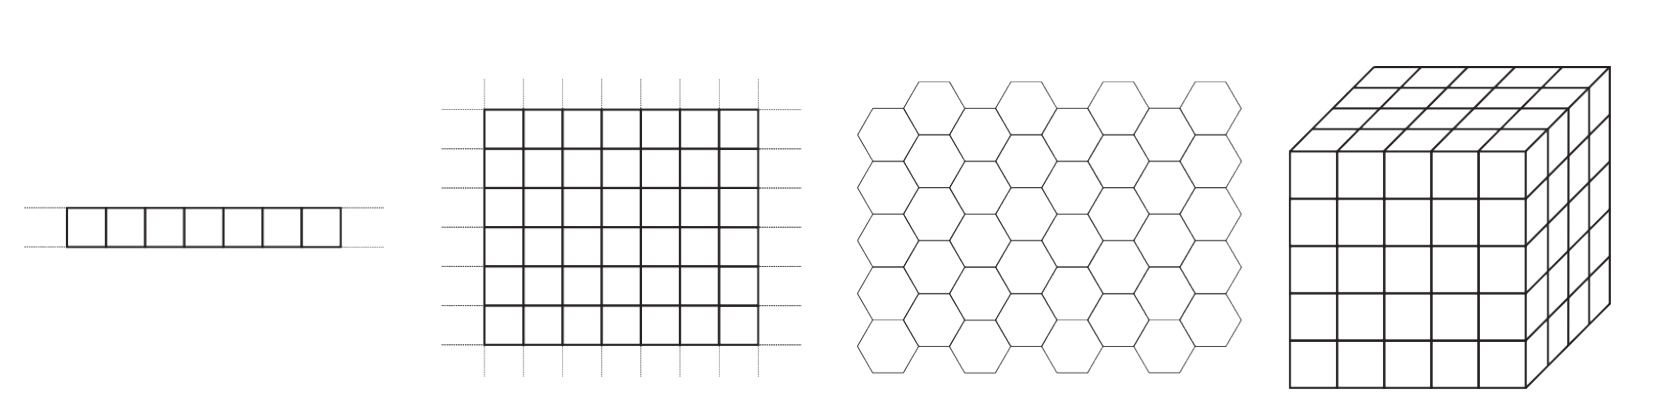
\includegraphics[width=\textwidth]{images/CA}
\end{figure}
}
%%%%%%%%%%%%%%%%%%%%%%%%%%%%%%%%%%%%
\frame{\frametitle{Cellular Automata}
	\begin{itemize}
		\item at time $t=0$ the state of the cells define the \textbf{initial conditions} of the CA
		\item All cells change state \textbf{simultaneously} (i.e. in parallel) at discrete time steps by means of the cell state \textbf{transition function}
		\item State transition function takes as input the states the cell's \textbf{neighborhood}
	\end{itemize}
	\begin{figure}
		\centering
		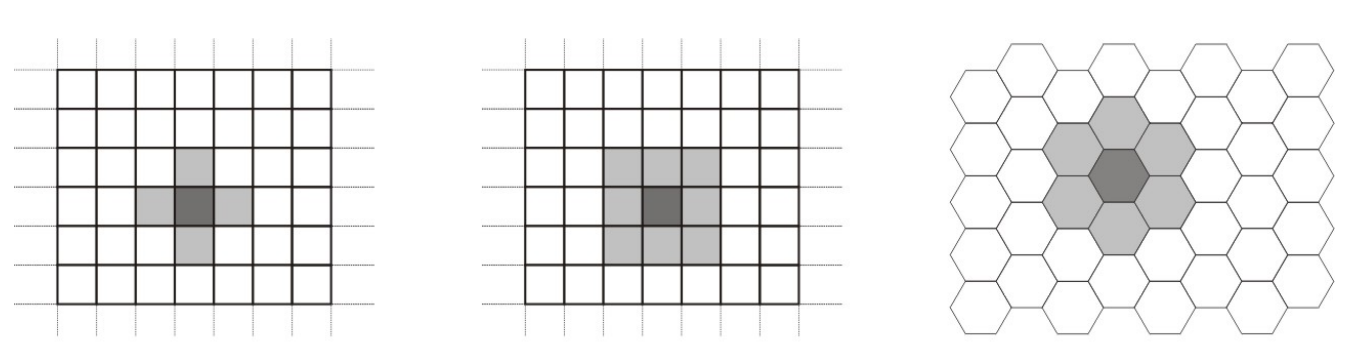
\includegraphics[width=\textwidth]{images/neighborhood}
	\end{figure}
}
%%%%%%%%%%%%%%%%%%%%%%%%%%%%%%%%%%%%
\frame{\frametitle{Cellular Automata}
	\begin{itemize}
		\item CA are simple but the complexity emerges even when the transition function is almost trivial
		\item A well known example is the \textbf{Conway's Game of Life}, that has been proven to be a Turing-complete computational system\footnote{P. Chapman. Life Universal Computer, 2002}.
	\end{itemize}
	\begin{figure}
		\centering
		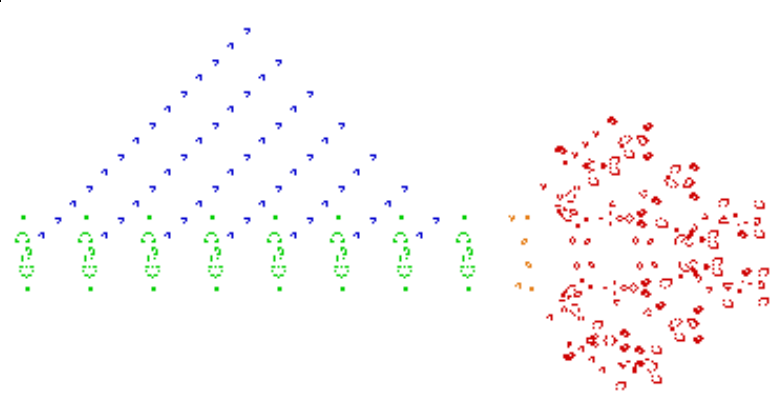
\includegraphics[width=\textwidth]{images/life}
	\end{figure}
	
}

%%%%%%%%%%%%%%%%%%%%%%%%%%%%%%%%%%%%
\frame{\frametitle{Cellular Automata}
	\begin{itemize}
		\item Widely Adopted in modeling and simulation
		\item Lattice Gas and Lattice Boltzmann simulation
		\item Fluid dynamics including macroscopic systems e.g. lava-flow,landslides 
		\item crowd dynamics, growth of crystals, etc.
	\end{itemize}
	\begin{figure}
		\centering
		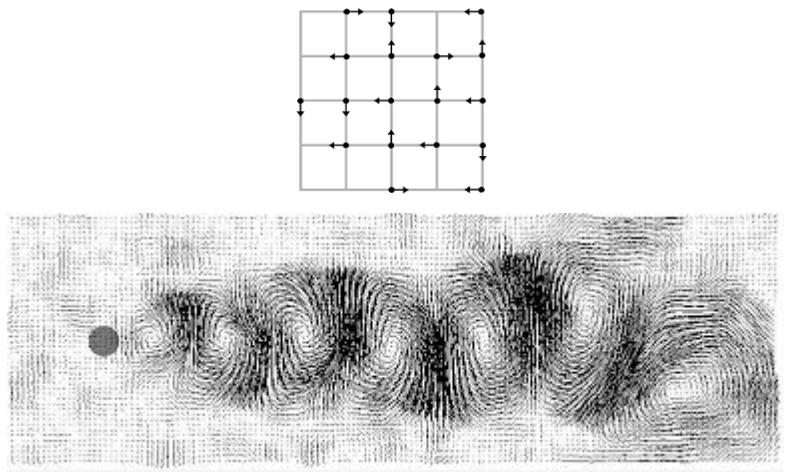
\includegraphics[width=0.85\textwidth]{images/boltzmann}
	\end{figure}
	
}


%%%%%%%%%%%%%%%%%%%%%%%%%%%%%%%%%%%%
\subsection{Finite Difference Method}
\frame{\frametitle{Finite Difference Methods}
	\begin{itemize}
		\item A method for solving Differential Equation (DE) Numerically
		\item Discovered by L. Euler and refined by Runge in 1910
		\item A DE is an equation where the unknown is a function
		\item e.g. Heat Equation: $\rho c\frac{\partial T}{\partial t} - \kappa \nabla^2T +Q=0$
		\item Boundary/Initial conditions are necessary e.g. temperature field at $t=0$
	\end{itemize}
\begin{figure}
	\centering
	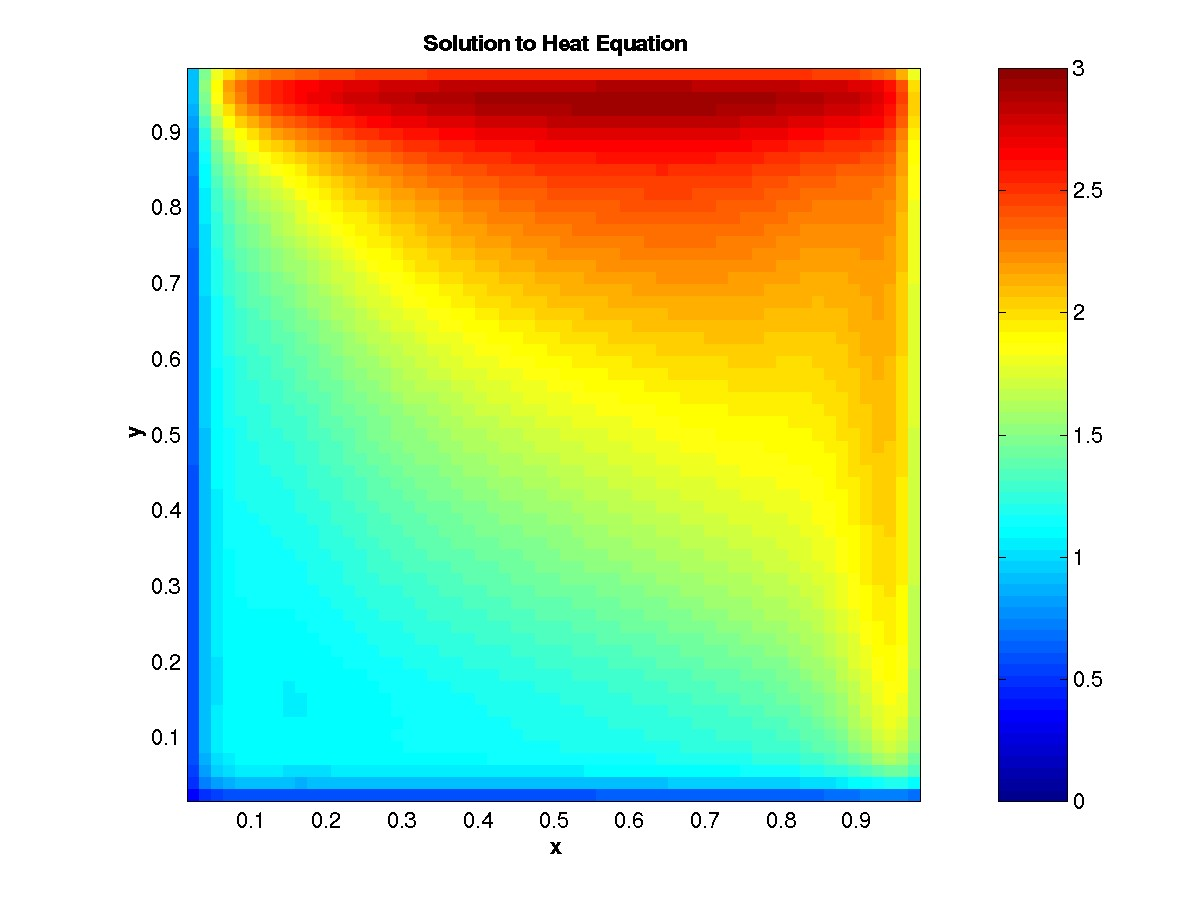
\includegraphics[width=0.65\textwidth]{images/heat2d_bc}
\end{figure}
	
}

\frame{\frametitle{Finite Difference Methods}
	\begin{itemize}
	
		\item Differential operator is \textbf{approximated locally} using \textbf{finite number of values}
		\item Domain is partitioned in a grid-like fashion
		\item Solution is computed for the grid points only
	\end{itemize}
	\begin{figure}
		\centering
		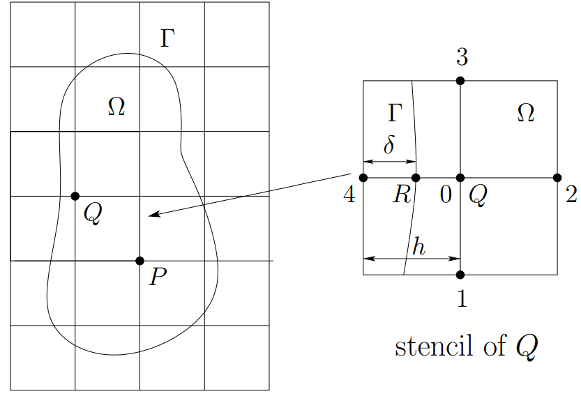
\includegraphics[width=0.8\textwidth]{images/gridcustom_shape2}
	\end{figure}
	
}

\frame{\frametitle{Finite Difference Formulas}
	\begin{itemize}
		\item Function approximating differential operator at a point using a finite number of neighbors
		\item Its arity determines the \textit{truncation order} of the formula
		\item The error is function of spacing between points in each direction 
		\item First order forward schema $\frac{\partial T(t,x)}{\partial x}  = \frac{T^n_{j+1} - T^n_{j}}{\Delta x} + \mathcal{O}(\Delta x)$ is obtained from: 
		 \[
		 T^n_{j+1} = T^n_{j} +
		\frac{\partial T}{\partial x}\bigg\rvert^n_j \Delta x +
		\frac{1}{2!}  \frac{\partial^2 T}{\partial x^2}\bigg\rvert_j \Delta x^2 + \ldots + 
		\frac{1}{k!}  \frac{\partial^k T}{\partial x^k}\bigg\rvert_j \Delta x^k + \ldots
		\]
		truncating at $k=1$ and solving for $\frac{\partial T}{\partial x}$

	\end{itemize}
}

\frame{\frametitle{Finite Difference Approximation of The Heat Equation}
	Given the initial value problem: $	\frac{\partial T(t,x)}{\partial t}=\kappa\frac{\partial^2 T(t,x)}{\partial x^2}$
\begin{itemize}
	\item Discretize the domain in a  1D regular uniform mesh
 	\item  first and second order derivative are substituted by forward and central difference formulas, respectively.
	\item Solving for $T^{n+1}_{j}$ leads to (explicit formula)
	\[
		 T^{n+1}_{j} = T^n_{j} + \frac{k \Delta t}{\Delta x^2} (T^n_{j+1}+T^n_{j-1}-2T^n_{j})
	\]
	\item The value for point at space coordinate $j$ at time $n+1$ can be obtained by using values of neighboring points i.e. $T^n_{j+1},T^n_{j-1},T^n_{j}$
\end{itemize}
}


